% ------------------------------------------------------------------------
% -*-TeX-*- -*-Hard-*- Smart Wrapping
% ------------------------------------------------------------------------
\def\baselinestretch{1}

\chapter{Analysis and Requirements Specification}

\def\baselinestretch{1.44}

%%% ----------------------------------------------------------------------

This chapter describes the details analysis and specification requirements for my dissertation project. 

\smallskip

%%% ----------------------------------------------------------------------
\goodbreak
\section{Proposed Solution}
Based on the findings of the literature analysis, it is clear that the healthcare industry is always looking for new ways to enhance customer service and boost service delivery via the use of cutting-edge technology. The proposed solution is to create a intelligent web portal that will
\begin{enumerate}[label=\arabic*)]
	\item show dementia related informations in categorized order,
	\item hold a chatbot in order to help users with their dementia related answers in a manner like a human conversation, 
	\item have a community forum to discuss about dementia related topics.
\end{enumerate}

The web portal will be routed to several pages which will show infromations about dementia, learning for dementia, technological solutions for dementia, and dementia related news and articles. The feasibility of incorporating a chat bot into applications has expanded as a result of developments in artificial intelligence, machine learning methods, higher aptitude for decision making, and a bigger availability of data. The user's question will be recognised and comprehended by the chatbot, and it will then come up with an acceptable answer depending on the overall context of the interaction. The portal will also connect the forum, where user will able to sign up, sign in, create post, and see the categorized posts.

\section{Information Collection}
This project is supported by Socitm (https://socitm.net/). Socitm is the UK’s leading
membership organisation of more than 2,500 digital and IT professionals helping shape and
deliver public services, with links to current work supporting people with dementia in Suffolk and Norfolk, the Building Research Establishment and a number of academic institutions. After meeting with them they provided initial requirements for the information related dementia care in the portal. As they didn’t have any kind of collected datasets, collecting information is one of the major tasks in this project. When someone in the family starts to suffer with dementia, then family members are totally unprepared, any support that one can find, any learning that exists and other people’s experiences and views are very valuable. Caregivers, be they professionals, family, friends etc. would benefit from a portal that contains: products, suppliers, and learning. These are the key area to be covered in the portal. 

There are many emerging technologies such as:
\begin{enumerate}[label=$\ast$]
	\item fall monitoring sensors
	\item community alarm systems that could be worn on the person (linked wirelessly) that were used for both monitoring and response in emergency
	\item door entry systems using voice, video, or both
	\item sensors linked to doors to make sure that the individual was moving around their home
	\item sensors linked to fridges, kettles, and other devices to monitor their use (and sometimes their contents)
	\item hearing loops
	\item at home medical support and diagnosis
	\item use of technology to keep people in touch with friends and relatives
	\item monitoring attendance in the home of external visitors including professionally sourced caregivers
	\item use of video within the home for safety and security although these technologies pose challenges in terms of privacy and appropriate use.
\end{enumerate}

The dataset is sort of collated information collected from background research and google search that: listed available technologies, who they might be available from, whether they had been used successfully (absence of review mechanisms), what costs there were, examples of best practice with balanced assessment of what had gone well/badly, ease of use, appropriateness, opportunities for collaborative approaches across both private and public sectors.

\section{Software Development Strategy}
It is essential to make a decision about a suitable methodology before beginning the advancement of any software programme. This will guarantee that a reasonable timetable is created for each step of the project and that needs are described in a concise manner. During the process of developing and designing this programme, a number of different development approaches will be examined and taken into consideration. As an offshoot of the waterfall model, incremental model of the software development methodologies came along. Design, development, and testing of the application all occur in incremental steps \citep{ana1}. Each build will culminate in the production of a new module or feature. 

\begin{figure}
	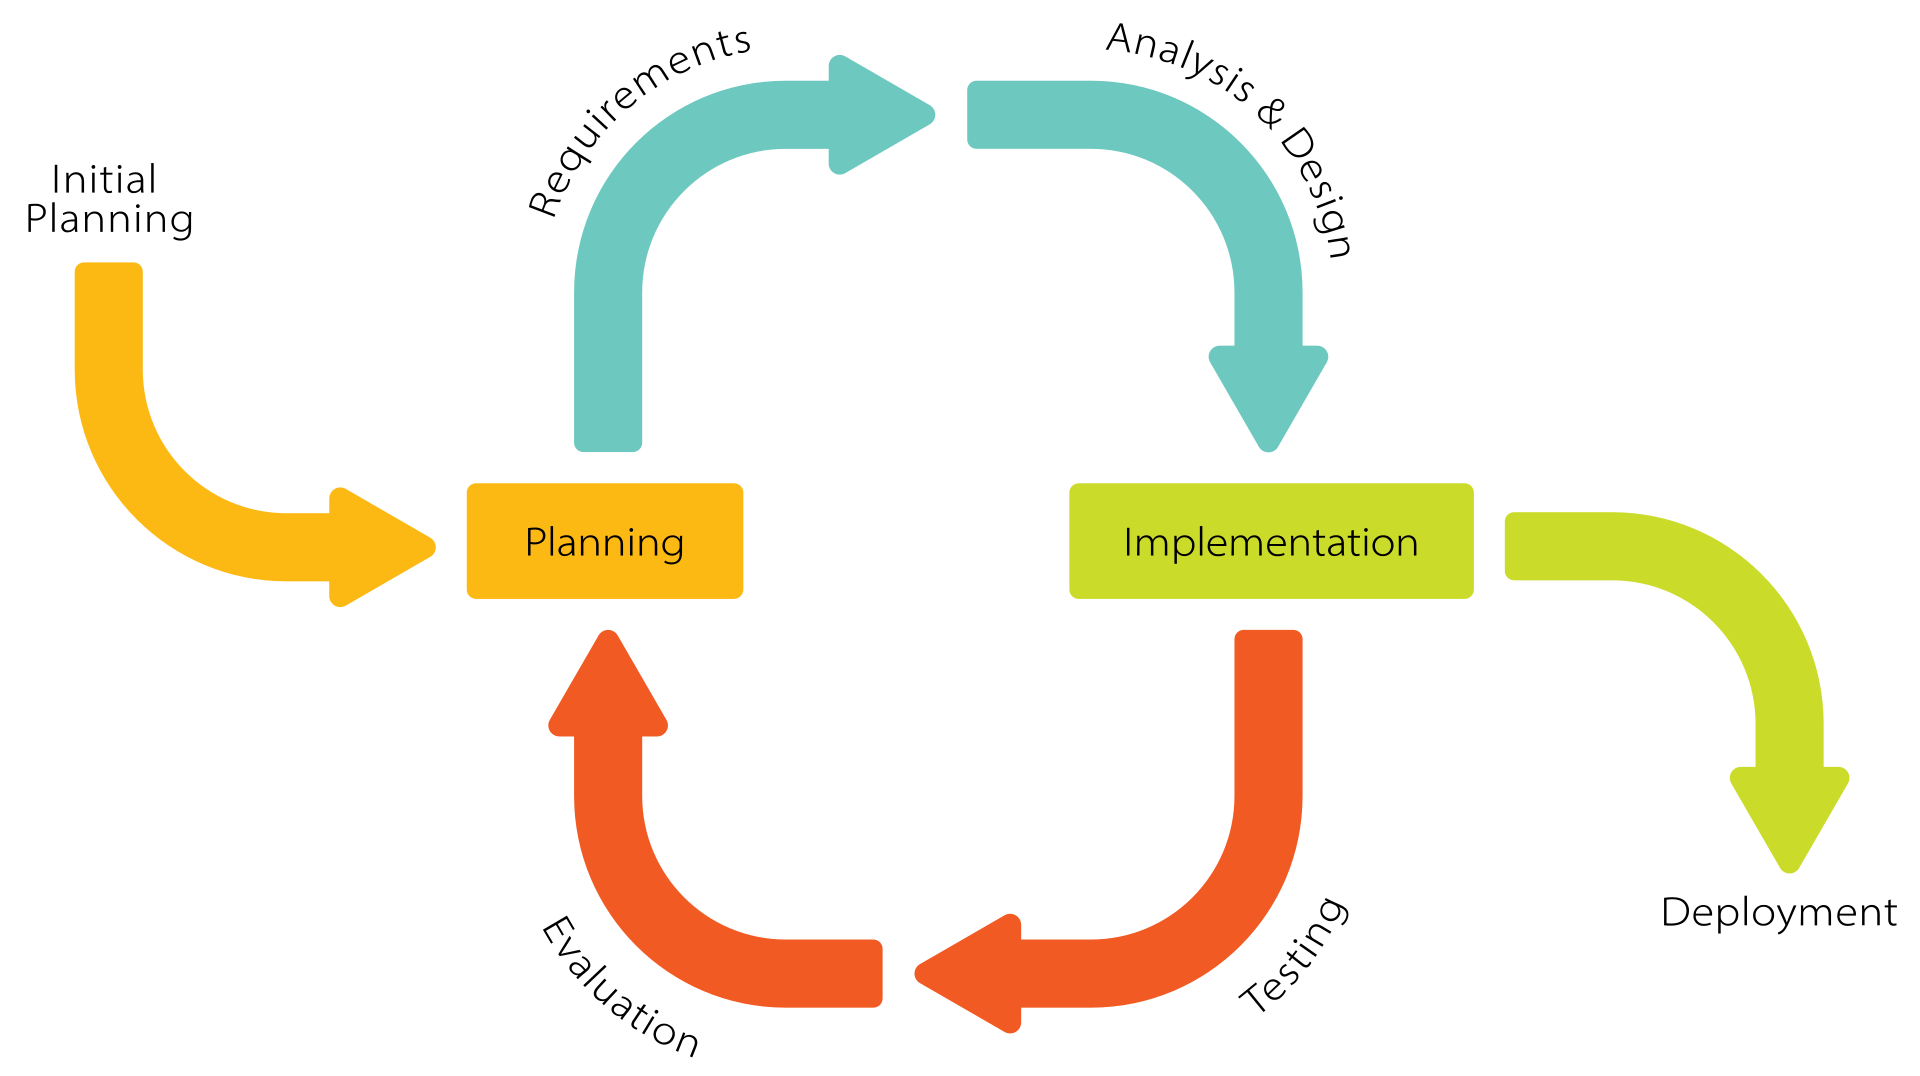
\includegraphics[width=\linewidth]{incremental}
	\caption{Incremental Model Overview.}
	\label{fig:2}
\end{figure}

Figure \ref{fig:2} displays the incremental model methodology. The project's complexity will increase as new needs are found and included into each incremental build, building on the features introduced in earlier versions. Early fault detection in brief cycles simplifies testing and troubleshooting. This project should use incremental development. Each successive build makes it straightforward to integrate new needs during the development process, making the incremental approach perfect for this project. 

\section{Software and Hardware Specifications}
Listed below are the software and hardware prerequisites that must be met in order to successfully build the web portal with chatbot and forum.
\subsection{Software Requirements}
\begin{enumerate}[label=$\bullet$]
	\item Operating System: Windows or Linux
	\item Front-end: HTML, CSS, Bootstrap, Javascript
	\item Back-end: Python
	\item Browser: Mozilla Firefox, Google Chrome
	\item Django
	\item Flask
	\item Visual Studio Code
	\item SQLite
	\item nltk
\end{enumerate}
\subsection{Hardware Requirements}
\begin{enumerate}[label=$\bullet$]
	\item Processor: Intel Core i3 (minimum) 
	\item Ram: 2 Gb (minimum)
	\item Hard drive: 50 Gb
\end{enumerate}

\section{Project Planning}

While a list of work progress outlining the project breakdown is created to serve as a management plan to be adhered to over the project lifespan, modest modifications may be made in each iteration as certain requirements may need to be modified. Project deliverables have their own individual checklists of tasks to be taken throughout each iteration. Create a Gantt chart outlining the semester-by-semester project activities and a risk management strategy.

\subsection{Project Milestones}
The project's progress is evaluated using the milestones, which also serves to establish due dates for activities and reveal which goals have been attained. Table \ref{table:1} highlights the project milestones.

\begin{table}[!h]
	\centering
	\begin{tabular}{ |c|c|c| } 
		\hline
		Milestone & Milestone Description & Completion Date \\
		\hline
		1 & Literature Review & 25.05.2022 \\ 
		2 & Analysis & 06.06.2022 \\ 
		3 & Design & 20.06.2022 \\ 
		4 & Iteration 1 & 01.07.2022 \\
		5 & Iteration 2 & 16.07.2022 \\
		6 & Iteration 3 & 27.07.2022 \\
		7 & Final Iteration & 08.08.2022 \\
		8 & Testing & 15.08.2022 \\
		9 & Evaluation & 21.08.2022 \\
		\hline
	\end{tabular}
	\caption{Project Milestones.}
	\label{table:1}
\end{table}

\subsection{Project Work Breakdown}
To ensure the project's success while using an incremental approach, it's crucial to define what features must be included throughout each iteration. In the event that new necessities emerge during development, they will be included into an ongoing iteration if they are manageable, or a new variant would be introduced to the schedule if they are substantial. Table \ref{table:1} shows the detailed iterations of the project.
\begin{table}[!h]
	\centering
	\begin{tabular}{|c|p{10cm}|} 
		\hline
		Iteration & Functional Implementation \\
		\hline
		Iteration 1 & \begin{itemize}[label=$\ast$] 
			\item Install and make a Django app
			\item Develop a homepage
			\item Develop four connecting pages
		\end{itemize} \\ 
		\hline
		Iteration 2 & \begin{enumerate}[label=$\ast$]
			\item Install and make flask app
			\item Make intent JSON file
			\item Train knowledge base model
			\item Implement standalone chatbot
			\item Enable cross-origin resource sharing
			\item Connect chatbot to the main site
		\end{enumerate} \\ 
		\hline
		Iteration 3 & \begin{enumerate}[label=$\ast$]
			\item Develop a forum  site
			\item Add sign in and sign out
			\item Implement create, delete, and update post
			\item Implement comment section
		\end{enumerate} \\ 
		\hline
		Final Iteration & \begin{enumerate}[label=$\ast$]
			\item Integrate forum to the main site
			\item Necessary bug fixing and update
		\end{enumerate} \\
		\hline
	\end{tabular}
	\caption{Project Iterations.}
	\label{table:2}
\end{table}

When each cycle has been completed, the final answer will have been produced. The project is going to be reviewed so that the lessons learned may be highlighted, and reflection will be done on the full project life cycle. This provides me with the chance to talk about what was accomplished as well as the processes or aspects of future projects that I would approach differently as a result of the lessons I learned from this experience.

\subsection{Risk Management}
A critical part of minimising the effects of potential hazards on a project's overall success is determining and controlling the risks and consequences connected with the project. Prevention measures may be implemented to reduce the possibility of a risk arising if its potential effects are known early in the project's development. Github will be used to back up code and avoid loss, individual initiative will be used to stay on top of the project plan, the project report and critical documents will be backed up on a regular basis, and if an unanticipated day off happens, the lost work will be made up for.

\subsection{Project Management}
A Gantt chart that was made in online gantt chart maker and displays the timetable for the project can be seen below in Figure \ref{fig:3}. It is possible to determine once the project milestones need to be finished by using Gantt charts, which helps ensure that the work is completed on time. The following chart provides a summary of the tasks, as well as the sequence that they are going to be contested and the amount of time allocated to each activity.

\begin{figure}[h!]
	\centering
	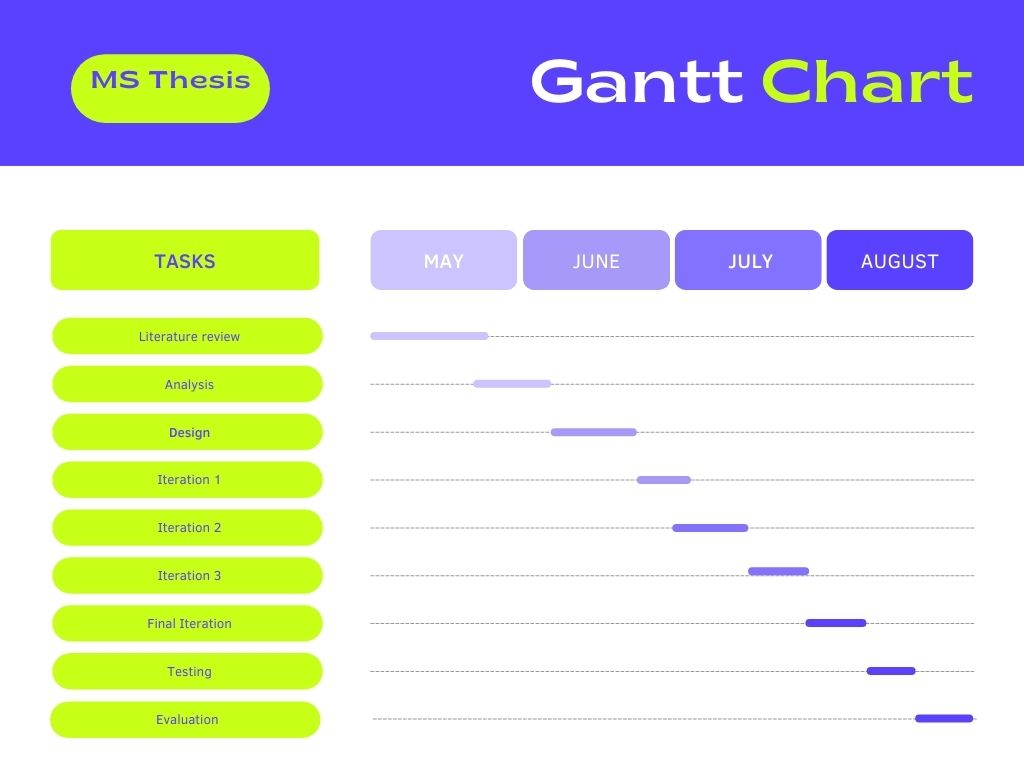
\includegraphics[width=0.8\textwidth]{gantt}
	\caption{Gantt chart for the project.}
	\label{fig:3}
\end{figure}

\def\baselinestretch{1.66}
\medskip

%%% ----------------------------------------------------------------------
